\section{Program Functionality}
	\subsection{Main Program Execution}
		The functionality that was achieved solves a 2D domain with a variety of obstacles and goals, however the program can easily be extended into 3 dimensions. The code solves for paths that avoids stationary obstacles given the origin point and any number of goal shapes. 
		There are five main classes that are implemented in this code:
		\begin{enumerate}
			\item ParseDataJSON
			\item Domain
			\item Solution
			\item Results
			\item Plot
		\end{enumerate}
		These classes are all used in the core file that executes the program (path\_planner.py). The user defines the parameters used for the entire code in one input .json file that gets parsed and fed into the Domain and Solution classes. The domain and solution objects are then used in the Results and Plot classes to save the .txt file of the results and a final interactive .html plot.  
	
	
	\subsection{Design Features Implemented}
		A domain can be defined using a rectangle or circle. The domain is only plotted if it is a circle, in a black line. At this time, freeform domains are not implemented, but if the user would like to modify the boundary of the domain, freeform obstacles can be placed along the boundary. 
		
		The obstacles are all plotted as black shapes. The origin point is highlighted in orange and the goal shapes are in green. If the user wants a goal to be a point, then a circle can be used with a small radius. The obstacles and goals can either be regular shapes such as circles and rectangles, or freeform shapes using Portable Bitmap Image files. 
		
		The code currently can solve this path planning problem using either the Basic RRT or RRT Star algorithm. The RRT Star algorithm rewires the path in order to minimize the cost after each vertex is added. This can be seen in the examples below, as the edges of the graph are all oriented towards the goals instead of branching in random directions. The straighter paths in the whole network from the RRT Star algorithm effectively minimize the cost (distance) of the solution and can theoretically reach the optimal solution. This added accuracy in the solution comes at a higher computational cost, as there are added computations needed for rewiring the graph.  
		
		The code was run under many different scenarios; two of which will be highlighted below. The final plots also serve to validate the code visually. 
		
		Future work includes implementing the algorithm in 3D, adding other forms of input for the definition of freeform shapes, including a freeform domain, and creating animations of the plots. 
	
	\subsection{Working Examples}
		\subsubsection{Simple Rectangular Domain}
		
		The following example utilizes a rectangular domain with a relatively small number of trials. In order to illustrate the versatility of the code, there is an obstacle of each type, as well as two goals, one of which is freeform. As seen in the figure below, The algorithms correctly sample points within the complex freeform obstacle shape.   
		
		The input file for the Basic RRT is shown below. The only difference between the two input files is that instead of "rrt\_basic" the user would specify "rrt\_star".
		
		
		\verbatiminput{links/rectangle_mixed_goals_obstacles_basic.json}
		
		
		\begin{figure}[H]
			\centering
			\begin{minipage}[b]{0.4\textwidth}
				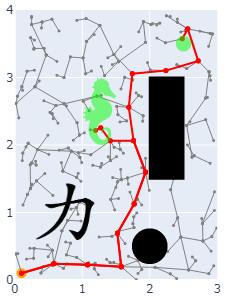
\includegraphics[width=\textwidth]{links/rectangle_basic.png}
				\caption{RRT Basic.}
			\end{minipage}
			\hfill
			\begin{minipage}[b]{0.4\textwidth}
				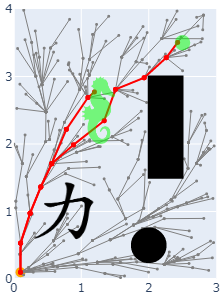
\includegraphics[width=\textwidth]{links/rectangle_star.png}
				\caption{RRT*.}
			\end{minipage}
		\end{figure}

The results text file would look like this: 
\verbatiminput{links/rectangle_mixed_goals_obstacles_basic.txt}

The Solution Path(s) are a list of the indices of the vertices that make up the solution path in order. The Solution Vertices are then printed such that the user does not need to search through the entire list of vertices to get the solution coordinates. The Solution Vertices lists the coordinates of the vertices corresponding to the solution path. Finally, the cumulative cost for the solution path is printed. If a solution is not found given the specified number of trials, then nan will be printed for all three fields. 

The table below summarizes the total costs for the solutions found using the two different algorithms.

		\begin{table}[H]
	\centering
	{\tabulinesep=2.0mm
		\begin{tabu}{ccc}
			\hline
			Solution Path & Basic RRT (Cost)     & RRT* (Cost)          \\ \hline
			1             & 26.093 & 12.571 \\ \hline
			2             & 45.169 & 24.916 \\ \hline
		\end{tabu}
	}
	\caption{\label{tab:rectangle_cost}Total cost (distance) for each solution using the Basic RRT algorithm versus the RRT* algorithm.}
\end{table}

\subsubsection{Complex Circular Domain}

This next example utilizes a circular domain with a large number of trials. There are obstacles and goals of each type. The large number of trials allows for the RRT* algorithm to find a very efficient solution, one that is almost a perfectly straight line.


		\begin{figure}[H]
	\centering
	\begin{minipage}[b]{0.4\textwidth}
		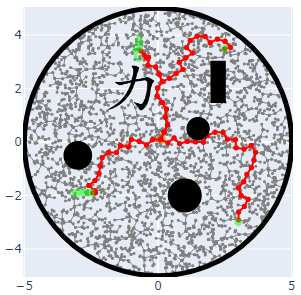
\includegraphics[width=\textwidth]{links/circle_basic.png}
		\caption{RRT Basic.}
	\end{minipage}
	\hfill
	\begin{minipage}[b]{0.4\textwidth}
		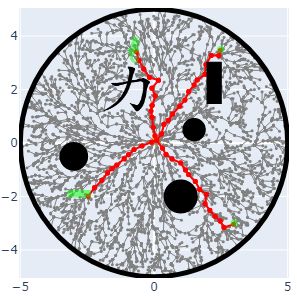
\includegraphics[width=\textwidth]{links/circle_star.png}
		\caption{RRT*.}
	\end{minipage}
\end{figure}

The results of the costs of the solutions found with the two different algorithms are shown in Table~\ref{tab:circle_cost}. The following are the key takeaways:
\begin{enumerate}
	\item There is a significant decrease in the final solution cost from using the RRT* algorithm.
	\item The step size plays a large role in finding goals that are relatively small. Some vertices will be very close to the goal, but not count as a valid solution because it is not inside the goal and a longer path is chosen.
\end{enumerate}

\begin{table}[H]
	\centering
	{\tabulinesep=2.0mm
		\begin{tabu}{ccc}
			\hline
			Solution Path & Basic RRT (Cost)     & RRT* (Cost)          \\ \hline
			1             & 38.593 & 23.626 \\ \hline
			2             & 82.726 & 35.132 \\ \hline
			3             & 40.171 & 19.396 \\ \hline
			4             & 97.500 &  38.963 \\ \hline
		\end{tabu}
	}
	\caption{\label{tab:circle_cost}Total cost (distance) for each solution using the Basic RRT algorithm versus the RRT* algorithm.}
\end{table}

